\chapter[SCP-020 隐形霉菌]{
    SCP-020 Unseen Mold\\
    SCP-020 隐形霉菌
}

\label{chap:SCP-020}

\begin{figure}[H]
    \centering
    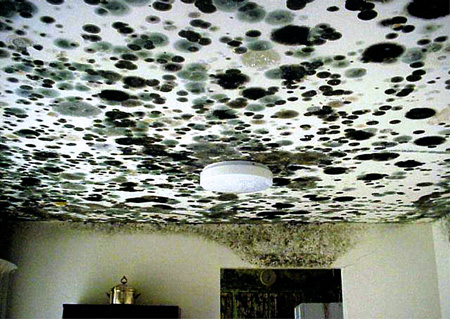
\includegraphics[width=0.5\linewidth]{images/SCP.020.jpg}
    \caption*{生长在平民居所的SCP-020}
\end{figure}

\bb{项目编号:} SCP-020

\bb{项目等级:} Keter

\bb{特殊收容措施:} SCP-020的样本被保存在一个密封的直径1米,高1米的圆柱形培养室中。这个培养室位于一个封闭的收容房间中,只能通过气密室访问。养分供应通过自动化的机器人系统管理,培养室在任何状况下都必须保持封闭状态。

密闭的视频监控摄像头安装在收容室,必须每天检查摄像头的完整性。进入收容室的任何人员在离开时都必须经过一个完整的抗真菌消毒程序。

\bb{描述:} 说明:SCP-020是一种快速传播的真菌,能够影响包括人类在内的所有生命物体的感官和行为。SCP-020的样本具有一个未知效应,使它们即使在显微镜下也无法被直接观察。只有通过摄像或监控,SCP-020才能被人类观察到。

一旦SCP-020,通常在人类居住地,构成菌落,它就会产生影响到它周围人类行为的孢子。受到影响的对象将提升其家园的温度和湿度,以创造出一个更适合SCP-020的生长环境。受影响的对象也变得更善于交际,在很多情况下,会经常邀请熟人到自己的家中,以进一步传播生命体。由于孢子和霉菌菌落是在无法察觉的情况下影响目标,霉菌有时可能会直接在活的主体上生长。

\begin{figure}[H]
    \centering
    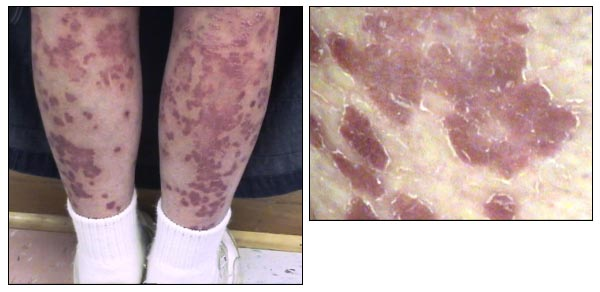
\includegraphics[width=0.5\linewidth]{images/SCP.020.2.jpg}
    \caption*{感染SCP-020菌落的平民}
\end{figure}

当一个家庭中的孢子和菌落到达临界浓度,受到影响的人类对象的健康会迅速恶化,并导致死亡。霉菌的进一步传播可能会发生在任何与死亡对象接触的急救人员和医疗人员之间,以及运送尸体到当地太平间的途中。

SCP-020的首次发现是在[刪除],当时一名SCP特工注意到当地医院的工作人员出现剧烈的性格改变。收容小组到达后,发现███名平民受到感染,相当于镇子上的大部分人。当地平民已被处决,镇子在当地一次短暂的森林火灾的掩护下被焚毁。

迄今为止,已有超过12例SCP-020爆发的报道。目前正在进行调查,以确定这些爆发的来源,并作出可能的预防措施。

\bb{附录020-01:} 从行动特遣部队Eta-10 ("See No Evil") 在[刪除]对SCP-020进行初步收容的音频\slash 视频的任务录像中摘录。

\begin{scpbox}

\bb{T2-领队:} 二组朝红色房子移动。\\\bb{T2-指挥:} 重复,无人机一号采集到一个热信号。

…

\bb{T2-领队:} 二组到位,准备br-[脏话]!\\\bb{T2-2:} 门打开了!

\ii{这时,一个平民女子出现在门口,她手里拿着菜刀。视频监控显示,她的脸近三分之二被霉菌覆盖着。}

\bb{平民女子:} 嗯……你们好,先生们……进来休息一会儿吗?\\\bb{T2-领队:} 趴在地上!丢掉武器!\\\bb{平民女子:} 别傻了!进来……待会儿……\\\bb{T2-领队:} 别动!丢掉武器!\\\bb{平民女子:} 我们……我们只是希望有一些客人……请……进来……\\\bb{T2-2:} 丢掉[脏话]武器!

\ii{推测在此时,受感染的平民注意到T2-4背着一个带引物的燃烧性武器,于是挥刀向队员扑来。}

\bb{平民女子:} [数据刪除]\\\bb{T2-领队:} 开火,开火!

\ii{枪声,尖叫。}

\end{scpbox}
